\documentclass[12pt]{article}


% Use the graphicx package for including images
\usepackage{graphicx}

% Use the hyperref package for clickable links within document
% and to webpages
\usepackage{hyperref}

% package for including snippets of code
\usepackage{listings}
% snippets of code are labeled Listing 1,2,...
% here changed to Algoritmus 1,2,...
\renewcommand{\lstlistingname}{Algoritmus}


%Use this package for theorems and proofs
\usepackage{amsthm}
\newtheorem{theorem}{Theorem}


\title{LaTeX} % title of the document
\author{J. Muravska} %your name
\date{} %today

% Start the text
\begin{document}
\maketitle
\tableofcontents


\section{Basic text formatting}

\LaTeX is a markup language in which we concentrate on highlighting
logical structure of the document. Normal text is written as
usual. Whitespace characters are treated as follows. \textbf{Multiple spaces}
mean the same thing as a single space. A single newline means the same
thing as a space, but an empty line is used to separate paragraphs.

This is the start of the second paragraph. 
Characters that have a special meaning in LaTeX
are inserted usually with backslash, e.g.~\verb'\%' is \%. Similarly
\$ is written as \verb'\$', \# as \verb'\#', \{ as \verb'\{'. Exceptions are @  written directly, \textbackslash{} as \verb'\textbackslash', $\sim$ written as \verb'$\sim$'.

Boldface and italics are introduced using commands
\verb'\textbf{some text}' and \verb'\textit{some text}'.  More about
fonts can be found in the corresponding
\href{https://en.wikibooks.org/wiki/LaTeX/Fonts}{Wikibooks chapter}.

\paragraph{Exercises} Make some words in this paragraph to appear in
italics and boldface. 

\section{Document structure}

Document starts with a preamble containing \verb'\documentclass'
command, various definitions and library imports. The text of the
document is located in an enviroment starting with
\verb'\begin{document}' and ending with \verb'\end{document}'.


Sectioning is done by commands \verb'\section', \verb'\subsection'
\verb'\subsubsection', \dots. The parameter of the command is the
title of the section. Bigger documents can also use \verb'chapter',
but then \verb'documentclass' should be changed from \verb'article' to
\verb'book'.  Command \verb'\paragraph' creates a heading located at
the start of the paragraph, followed by the text on the same line (see
an example in Section \ref{sec:details}).

The heading of the document can be produced using \verb'\maketitle'
command, and an automatically generated table of contents can be created
using \verb'\tableofcontents'.
For more details see the exercises
below.

Bulleted list are created using \verb'itemize' environment as
illustrated by the exercise below, numbered lists by \verb'enumerate'.

\paragraph{Exercise} 
\begin{itemize}
\item Add command \verb'\maketitle' after
  \verb'\begin{document}'. This typesets a title on the top of the
  first page using the information entered in the header of the document
  using \verb'\title', \verb'author' and \verb'date'. Try to fill in
  author and see how it appears.

\item Add a subsection somewhere in this document.

\item Add a command \verb'\tableofcontents' to the document, process
  the document twice with pdflatex to produce a correct table of contents.

\item Change this list of tasks from a bulleted to a numbered list.
\end{itemize}

\section{Mathematics}

Mathematical symbols or short expression placed directly in text are
placed between dollar signs, e.g. \verb'$x$' produces $x$.  Bigger
formulas are placed between \verb'$$' or in a special environment,
such as \verb'equation'.

There is syntax and macros for typesetting even complex mathematical
expressions. Examples can be found in Table \ref{tab:math}.
More information can be found in 
\href{https://en.wikibooks.org/wiki/LaTeX/Mathematics}{chapter from
Wikibooks}.

Definitions, theorems, lemmas etc.~can be typeset and numbered by
defining custom environments. Here is an example of a theorem.

$$\lim_{n\to\infty} \left( 1 +  \frac{1}{n} \right) = \e$$

\begin{theorem} If $x,y\ge 0$ then $\frac{x}{y}\ge 0$.
\end{theorem}

\begin{proof}This is so obvious that I do not now how to prove it.
\end{proof}

\begin{table}
\begin{center}
\caption{Examples of common mathematical notation}\label{tab:math}
\renewcommand{\arraystretch}{1.5}

  \begin{tabular}{@{}lll}
    \hline
    Commands & Result & Note \\
    \hline
  \verb'$x_1$' & $x_1$  & subscripts\\
  \verb'$x^2$' & $x^2$  & superscripts\\
  \verb'$x_{j+1}^{10}$' & $x_{j+1}^{10}$  & \{  \} needed here\\
  \verb'$\alpha, \Delta$' & $\alpha, \Delta$ & greek letters\\
  \verb'$\log_2 n$' &  $\log_2 n$ & many special functions available\\
  \verb'$log_2 n$' &  $log_2 n$ & ugly, use the form above\\
  \verb'$\sum_{k=1}^n k$' & $\sum_{k=1}^n k$ & sum ($\prod$ also available)\\
  \verb'$\{1,2,\dots, n\}$' & $\{1,2,\dots, n\}$ & note \verb'\dots' and \verb'\{'\\
  \verb'$\left(\frac{n}{k}\right)$' & $\left(\frac{n}{k}\right)$ & fraction, bigger parentheses \\
  \verb'${n \choose k+1}$' & ${n \choose k+1}$ & binomial coefficients \\
  \verb'$x\cdot y\le z$' &  $x\cdot y\le z$ & multiplication, inequality\\
  \verb'$x*y <= z$' &  $x*y <= z$ & ugly, use the form above\\
  \verb'$A\cup B\cap C$' & $A\cup B \cap C$ & set notation\\
  \verb'$A \setminus \emptyset$' & $A \setminus \emptyset$ & \\
  \verb'$A \subseteq B$' & $A \subseteq B$ & \\
  \verb'$a \in A, a \notin B$' & $a \in A, a\notin B$ & \\
  \verb'$A\lor B\land C$' & $A\lor B \land C$ & logic\\
  \verb'$\neg A\Rightarrow B$' & $\neg A\Rightarrow B$ & \\
  \verb'$\foreach x \exists y$' & $\forall x \exists y$ & \\
  \hline  
\end{tabular}
\end{center}
\end{table}

\paragraph{Exercise}
\begin{itemize}
\item Typeset in mathematical notation that the limit of 1 + 1/n
  raised to the power of n tends to e as n approaches infinity.  Use
  commands such as \verb'lim', \verb'frac', \verb'to', \verb'infty'.
  Note that the first sentence of this exercise incorrectly uses
  mathematical symbols such as $e$ and $n$ without enclosing them in
  dollar signs.

\item Add \verb'newtheorem' definition of lemma to the top of the file
  similarly as we have theorem right now and then try to add a lemma
  to the text.
\end{itemize}

\section{Some typesetting details}
\label{sec:details}

\paragraph{Non-breaking space.}
Non-breaking space is written as \verb'~'. You can use it to avoid
having a single-letter word at the end of the line (type \verb'a~word'
instead of \verb'a word') or to avoid longer space after a dot which
does not represent the end of a sentence (such as \verb'e.g.~word'). 

\paragraph{Dashes.}
LaTeX provides three lengths of dashes. A single minus sign 
is used as minus sign and as a hyphen, e.g.~``memory-efficent'',
number -1.  An en dash, written as \verb'--', is longer and is used for
example for ranges, such as 11:30--13:00. Finally an em dash, written as
\verb'---', is used instead of colon or parenthesis in a sencence, such as ``We use efficient sorting algorithms---mergesort and quicksort.''

\paragraph{Quotes.} As you can see in the sentence above, English-language quotes are produced by two back-ticks \verb|``| at he beginning of a quoted text and two apostrophes  \verb|''| at the end.

In Slovak, macro \verb'\uv{text}' is used to correctly quote text. First Slovak language has to be switched as shown in Section \ref{sec:sk}.

\paragraph{Spacing and word division.} LaTeX has many macros for adding or decreasing spaces both horizontally and vertically. However, in most cases it is better to leave the layout of the text as is rather than make manual adjustments. LaTeX should correctly divide words at the end of lines, but if you want to suggest a different word break, use \verb'\-'. For example, \verb'im\-pos\-si\-ble' suggests three possible places where the word can be divided, and LaTeX will choose the one that fits best.\footnote{This is the correct division of the word according to the \href{https://www.merriam-webster.com/dictionary/impossible}{Merriam-Webster dictionary}. This is also an example of a footnote, but do not use too many footnotes in your text.}


\section{Figures and tables}

Figures can be included using \verb'\includegraphics' command.  In
formal technical texts, figures should be included in a \verb'figure'
environment and described using \verb'caption' command. An example of a figure (with a missing caption to be added as an exercise) is shown in Figure \ref{fig:triangle}.

\begin{figure}
  \begin{center}
    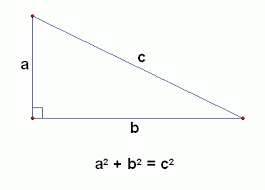
\includegraphics[width=6cm]{triangle.png}
  \end{center}
  \label{fig:triangle}
\end{figure}
    
Tables are created using \verb'tabular' environment.  Columns are
specified using justification left (l), center (c) or right (r),
e.g.~a table started with \verb'\begin{tabular}{llr}' will have two
left-justified columns and one right-justified. Columns are separated
with \verb'&' and rows with \verb'\\'. Tables should
be included in \verb'table' environment, as shown in Tables
\ref{tab:math} and 
\ref{tab:table}.

\begin{table}
  \begin{center}
    \caption{This is an example of a table. This text is the caption
      and should explain the meaning of the table. }
    \label{tab:table} % create a label for the table, after caption

    \begin{tabular}{lcr}
      \hline
      Left-justified column & Centered-column & Right-justified column \\
      \hline
      The first longer text & Another longer text & Another longer text\\
      Short & Short & \\
      \hline
    \end{tabular}
  \end{center}
\end{table}


\paragraph{Exercise}
\begin{itemize}
\item Add caption to the figure similarly as it is done in the tables. Figure caption should be below the figure but before the label command. 
\item Add another row to Table \ref{tab:table},
  which will have the first two columns
  merged into a single cell. This is achieved using command\\\
  \verb'\multicolumn{2}{c}{content of the merged cell}'
\end{itemize}
  
\section{References to parts of a document}

You can label various parts of the document using
\verb'\label{yourId}' command. Then refer to the section, figure,
theorem, equation, etc.~using \verb'\ref{yourId}'. This is one of the
most useful features of LaTeX.

\paragraph{Exercise}
Which parts of the document already have \verb'\label' command?
Add label to the theorem. Then refer to it. 

\section{Slovenčina}
\label{sec:sk}

%section 3
Ako funguje ľščťžýáíé a literatúra

Slovenčinu pridáme ľahko s použitím balíčkov inputenc a babel, ktoré
treba pridať do hornej časti dokumentu. Potom by mala fungovať
diakritika a namiesto anglických výrazov ako Table of contents by sa
mali objaviť slovenské.

\paragraph{Exercise} Pridajte do hornej časti nasledujúce príkazy:
\begin{verbatim}
\usepackage[utf8]{inputenc}
\usepackage[T1]{fontenc}
\usepackage[slovak]{babel}
\end{verbatim}

\section{Literatúra}

Na pridávanie literatúry do textu sa najčastejšie používa
BibTex. Jednotlivé detaily citácií si zhromaždíme do .bib súboru, na
ktorý sa potom vieme odkazovať pomocou cite.
Odkazy na literatúru robíme príkazom \verb'cite'.

\paragraph{Cvičenie}
\begin{itemize}
\item Na koniec súboru pred \verb'\end{document}' dajte príkazy
\begin{verbatim}
\bibliographystyle{plain}
\bibliography{literatura}
\end{verbatim}
\item V texte použite príkaz \verb'\cite{clanok}'. Pozrite si ID článkov v
  bib súbore a zacitujte ešte jeden ďalší pomocou \verb'cite'. 
\item Spustite príkazy
\begin{verbatim}
pdflatex tutorial 
bibtex tutorial
pdflatex tutorial 
pdflatex tutorial 
\end{verbatim}
Na konci dokumentu by sa mal objaviť zoznam citovanej literatúry.
\end{itemize}

\section{Algoritmy a zdrojový kód}

Kus kódu bez formátovania môžete dať do prostredia \verb'verbatim',
ktoré bolo použité aj v tomto dokumente. Krajšie je použiť prostredie
\verb'lstlisting' z balíčka \verb'listings', v ktorom môžete nastaviť
aj jazyk a kód bude krajšie sformátovaný (Algoritmus \ref{alg:C}).
Ak chcete mať pekne
sformátovaný pseudokód aj s matematickými výrazmi, môžete použit
balíček \verb'algpseudocode'. Dá sa to však aj v \verb'lstlisting',
kde môžete použiť nastavenie \verb'escapeinside={(*}{*)}' a potom
medzi \verb'(*' a \verb'*)' dávať Latexový kód, napr. matematické
výrazy.

\lstset{language=C,caption={Algoritmus na výpočet faktoriálu v jazyku C},label=alg:C}
\begin{lstlisting}
int factorial = 1;
for(int i = 1; i <= n; i++) {
    faktorial *= i;
}  
\end{lstlisting}




% tu by to asi chcelo tú literatúru
\end{document}

